\chapter{总结与展望}\label{chap:conclusion}

本章节主要对前面提出的创新点和工具实现进行系统的总结,归纳本工作主要的贡献,并讨论后续工作的可行性。

\section{工作总结}
SMT问题一直是形式化验证与软件工程领域的核心问题,SMT求解器在很多方面有着广泛的应用,很多验证算法最终都需要SMT求解器给出解答。非线性实数理论因为其约束的复杂性和无理数赋值的困难性,一直是SMT问题中的难点。以往的工作既有根据多项式胞腔理论设计的系统方法,也有从SAT问题借鉴而来的启发式方法,但是这些方法在实际应用中都有一定的局限性,在特定问题上表现不佳。本工作提出了一种针对非线性实数所有样例的局部搜索算法工具LS\_NRA。具体来说,其包含以下几部分组成:基于边界的胞腔跳跃分数缓存机制、等式约束松弛机制、非单变量操作的前瞻机制。实验表明,LS\_NRA在大多数情况下都能够在较短时间内找到解,并且相比于主流SMT求解器(Z3、cvc5)在高次约束上优势明显。

以往工作提出了用于算术理论的关键移动操作,针对非线性问题拓展成了胞腔跳跃操作。但是以往的工作只是针对单一子句而言,并没有基于变量级别的可行域来分析,造成了操作的冗余和迭代地低效。本工作首先提出了边界数据结构来模拟胞腔之间的间隔,基于此提出一种变量分数的增量式计算方法,而非传统的迭代计算,并且给出了边界信息的迭代条件和迭代信息,从而使得局部搜索单词计算量的下降和迭代性能的提升。

本工作的另一个创新点是针对等式约束的特殊处理。非线性实数理论是唯一一个涉及到无理数赋值的算术理论,这也是以往的局部搜索工作避开高次非线性约束的一个理由。本工作首先引入了赋值复杂度的概念,给出了赋值对迭代次数影响的分析,进而提出等式松弛机制,以暂时扩大可行域来增加赋值的可能性,从而提高了算法的求解能力。本工作还给出了两种恢复方法,即基于约束结构的传播机制和受限局部搜索,最终完成SMT问题精确解的搜索。

此外,本工作还探讨了实现细节。比如,本工作定义了无单变量操作的文字状态,并给出一种两种变量前后移动的前瞻机制,可以确保在给定的候选赋值中增加变量跳出停滞状态的可行性。此外,本工作还引入了两种重启机制,单一变量或所有变量的重新赋值方法,并规定在一定步数迭代没有效果时使用。最后,本工作详细阐述了LS\_NRA的不同实现组件,包括预处理部分、线性方程的快速计算和参数的选择。

基于上述思想,本工作测试了LS\_NRA在同一测试环境下与其他局部搜索算法和主流SMT求解器的求解能力。实验表明,LS\_NRA整体上要优于其他主流方法,并且在高次约束上表现最优。经过消融实验,我们证明了以上方法的有效性,并且给出了每个组件的重要性。

\section{未来展望}
\subsection{局部搜索算法的拓展}
本工作作为局部搜索算法在算术理论的拓展,对后面的工作有很多启发作用。首先,目前的缓存机制仍然是基于边界数据结构的单变量可行域执行的,但是在实际的解空间$R^n$中,同一胞腔内每个变量的可行域都是固定的,因此更好的解决方法是能够定位到当前遍历的胞腔序号,这样可以确保重复遍历带来的可行域重复计算问题。其次,目前对于等式约束的松弛算法很基础,复杂度阈值是一个预设的常数,但是在实际搜索过程中应该区别不同难度的等式约束,即为不同难度的等式约束设置不同等级的阈值条件。再者,前序工作的多变量移动机制涉及到参数方程的方向向量选定问题,目前的工作都是基于预设的几组方向向量,而非动态调整。一个启发式的创新是使用强化学习方法实时检测不同方向对搜索状态的作用,然后实时调整多变量的搜索方向。

\subsection{与完备算法的互补}
如章节\ref{chap:Result}所述,局部搜索算法往往在高次约束上表现甚好,而完备算法则在强推理性地样例上表现突出。工作\cite{CaiZ21,hybridSMT}分别提出了用于SAT和SMT问题的混合求解方法,目前已经成为SAT-COMP和SMT-COMP的主流求解方法。然而,目前的算法更多的还是和CDCL/CDCL(L)进行耦合,而非MCSAT算法。此外,本文提出的LS\_NRA基于胞腔的操作机制可以和MCSAT算法中的CAD解释相关联,比如在局部搜索遍历一个不满足胞腔时自动学习一个相关的引理。我们将目前和潜在的技术路线归纳在图\ref{fig:future}中。

\begin{figure*}[t]
    \centering
    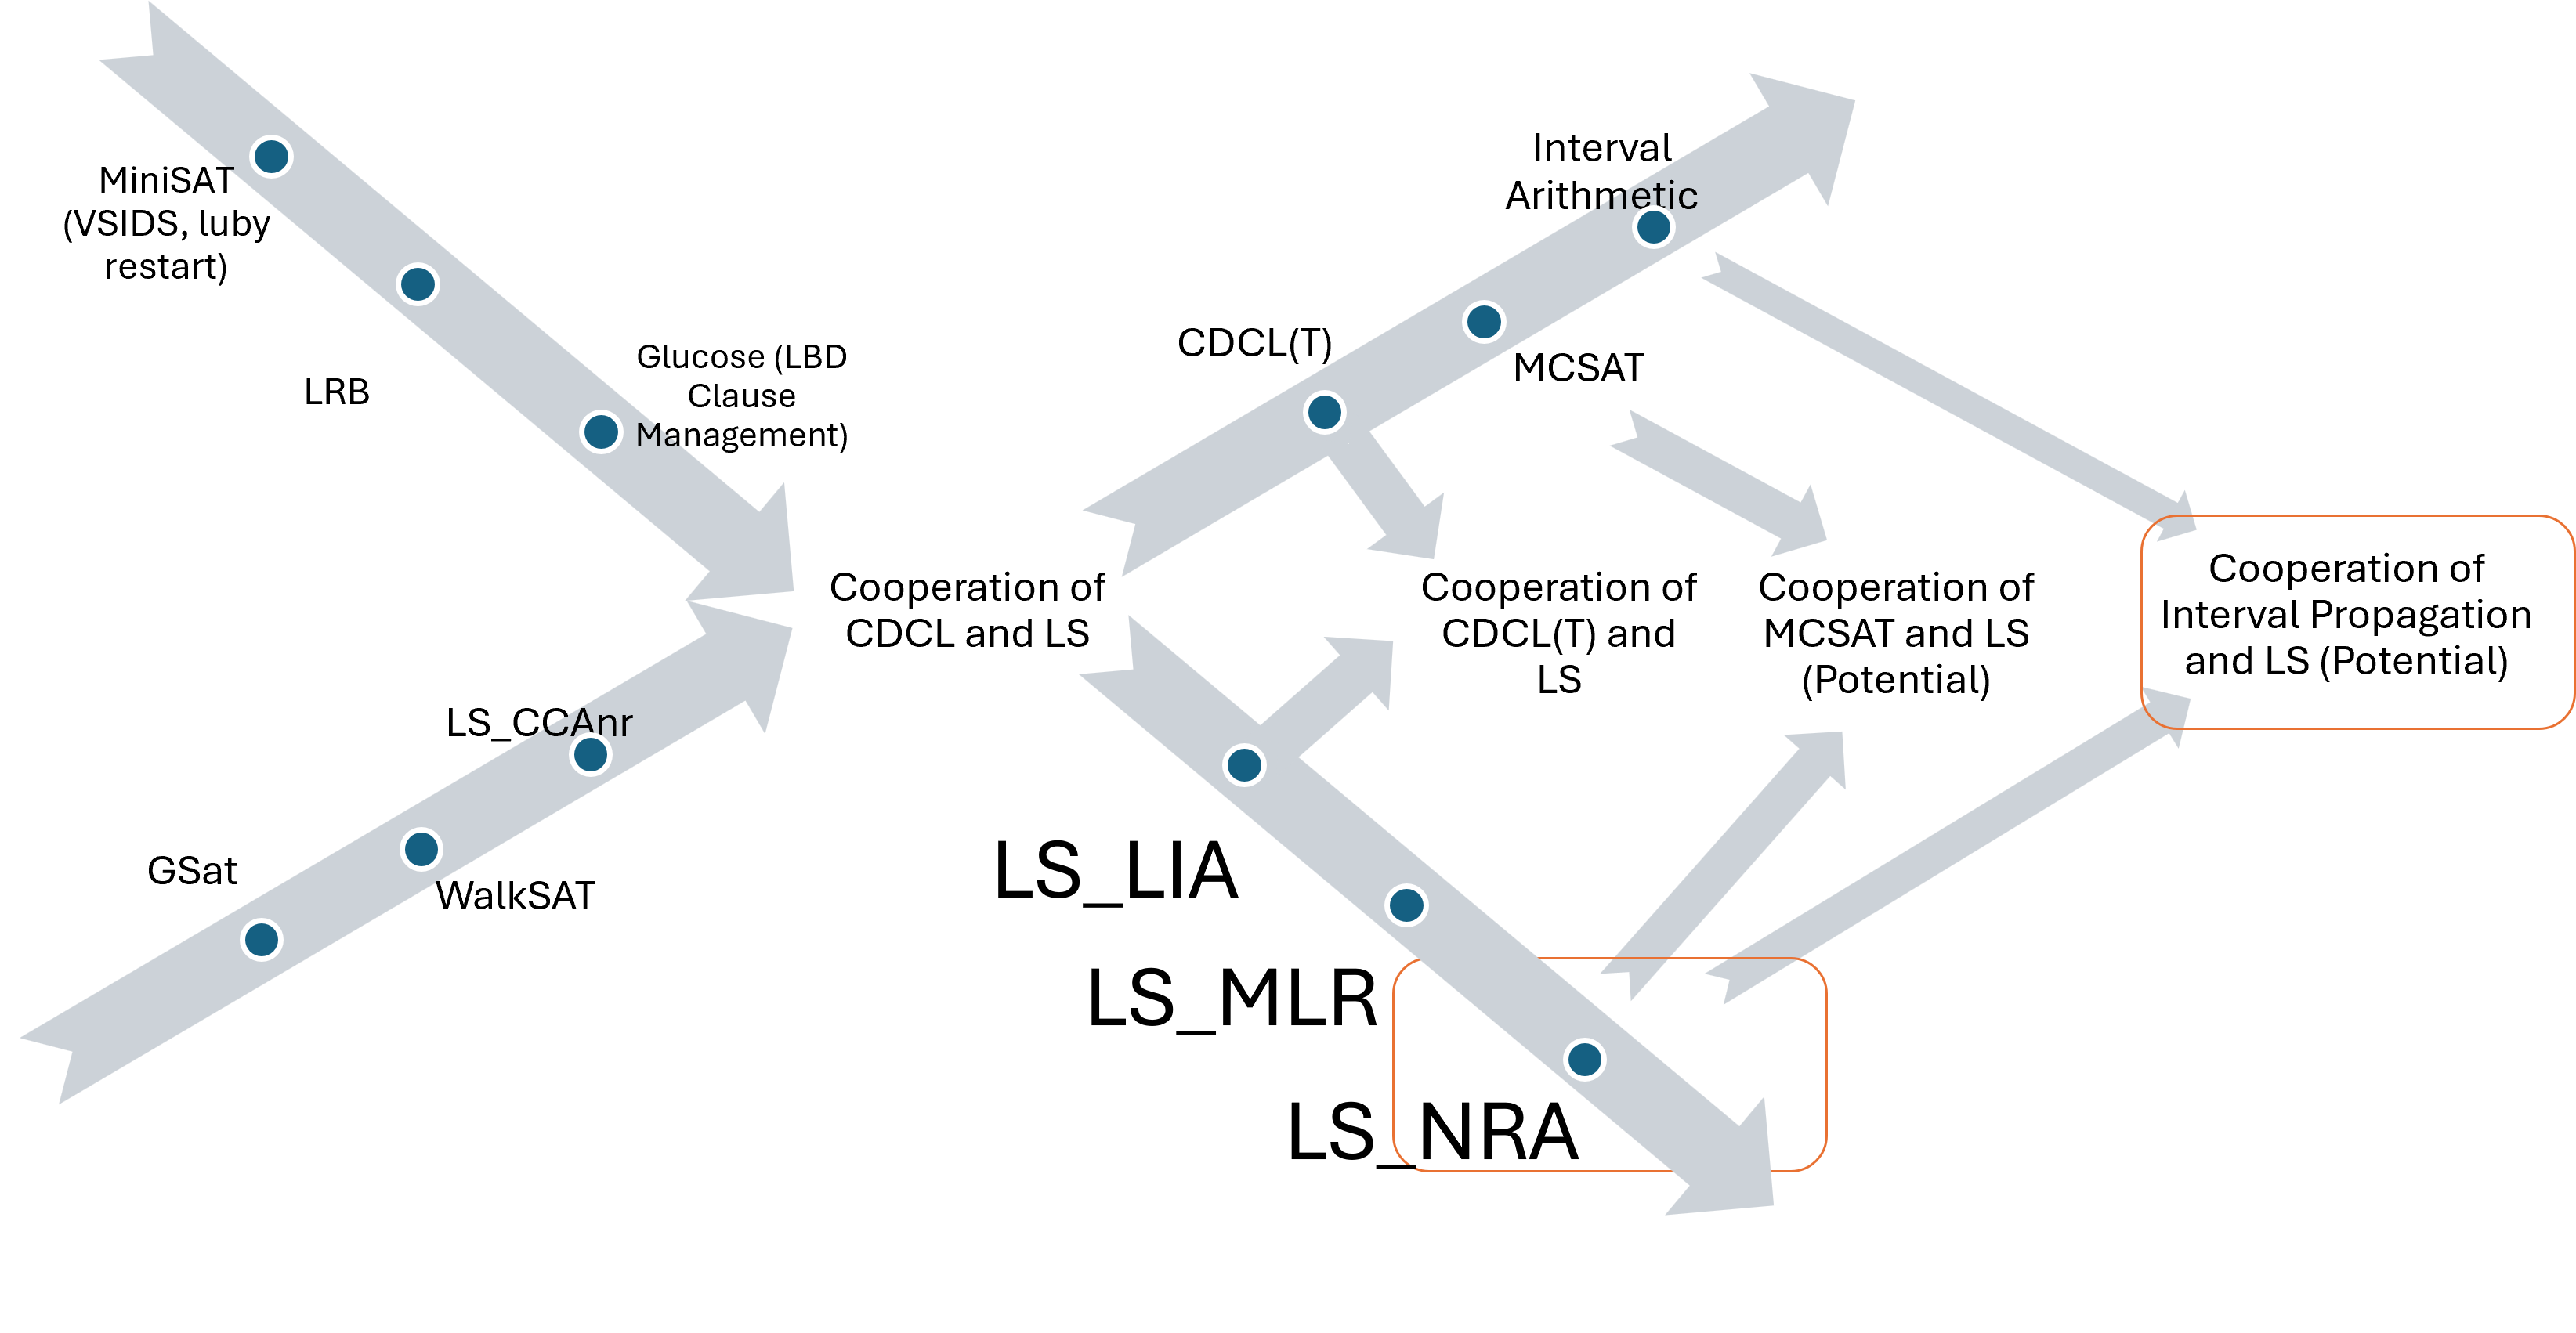
\includegraphics[width=\columnwidth]{Img/future.png}
    \bicaption {局部搜索算法和完备算法的主要技术路线。} {Main Technical Routes of Local Search Algorithms and Complete Algorithms.}
\label{fig:future}
\end{figure*}

\clearpage